\section{Funciones Medibles}
Comprobadas las propiedades que tiene la medida sobre conjuntos medibles, nos interesa saber qué funciones nos permiten conservar propiedades de medida interesantes. Es aquí donde juegan un papel fundamental las funciones medibles, que permiten asegurar que las preimágenes de abiertos son medibles y, por ello, al trabajar sobre abiertos no debemos preocuparnos sobre las propiedades de medibilidad ya que se conservan también en el conjunto de partida.
 
\begin{defi}
Sea $A \subset \mathbb{R}^n$ medible y $f: A \rightarrow \mathbb{R}^m$, definimos una función \textbf{medible} como aquella que verifica:
$$\forall G \subset \mathbb{R}^m \text{ abierto, } f^{-1}(G) \text{ es medible}.$$ 
\end{defi}

\begin{prop}
\begin{enumerate}
\item Sea una función $f: \mathbb{R}^m \rightarrow \mathbb{R}^m$, si es continua, entonces es medible.

\item Sea $f: A \rightarrow \mathbb{R}^m$ una función medible y $\varphi: \mathbb{R}^m \rightarrow \mathbb{R}^k$ una función continua\footnote{En general, la composición de medibles no tiene porqué ser medible}, entonces $\varphi \circ f$ es medible.
\end{enumerate}
\end{prop}

\begin{obs}
Como podemos expresar un abierto como recubrimiento de bolas (que con la norma infinito serían cubos) tenemos que $G = \bigcup_{k \in \mathbb{N}} Q_k$, de este modo, se tiene que $f^{-1}\left( G \right) = \bigcup_{k \in \mathbb{N}}f^{-1}\left( Q_k \right)$ y, en consecuencia, podemos redefinir el concepto de función medible de la siguiente forma:
$$f \text{ medible} \Leftrightarrow f^{-1}\left( Q \right) \text{ medible, } \forall Q \subset \mathbb{R}^m \text{ cubo abierto.}$$
\end{obs}


\begin{prop}
Sea $f: A \rightarrow \mathbb{R}^m$ una función, es medible si y sólo si cada una de sus componentes es medible.
\end{prop}
\begin{demo}
\begin{itemize}
\item $\Rightarrow$

Cada componente se puede expresar como:
$$f_i = \pi_i \circ f$$
Donde $f$ es medible por hipótesis y $\pi_i\left( x_1, \ldots, x_m \right) = x_i$ es continua.

\item $\Leftarrow$

Dado $Q = \left( a_1, b_1 \right) \times \ldots \times \left( a_m, b_m \right)$ cubo abierto, tenemos que $f^{-1}\left( Q \right) = \bigcap_{i = 1}^{m} f_i^{-1}\left( a_i, b_i \right)$. Esto es así porque:
$$x \in f^{-1}\left( Q \right) \Leftrightarrow f\left( x \right) \in Q \Leftrightarrow \forall i \in \mathbb{N} : f_i\left( x \right) \in \left( a_i, b_i \right)$$
\end{itemize}
\end{demo}

\begin{prop}
Sean $f, g: A\subset \mathbb{R}^n \rightarrow \mathbb{R}^m$ medibles, se cumplen las siguientes propiedades:
\begin{enumerate}
\item $f+g$ medible.
\item $\forall a \in \mathbb{R}: a\cdot f$ medible.
\item $\left<f, g\right>$ medible.
\item $\vert \vert f \vert \vert$ medible.
\end{enumerate}
\end{prop}
\begin{demo}
\begin{enumerate}
\item Definimos la función $F: A \rightarrow \mathbb{R}^{2m}$ de la forma:
$$F\left( x \right) = \left( f_1\left( x \right), \ldots, f_m\left( x \right), g_1\left( x \right), \ldots, g_m\left( x \right) \right)$$
Y por hipótesis, como las funciones son medibles y cada componente es medible, entonces $F$ es medible. Del mismo modo, definimos: 
\begin{align*}
+: \mathbb{R}^m \times \mathbb{R}^m & \rightarrow \mathbb{R} \\
\left( u, v \right) &\mapsto u+v
\end{align*}
que trivialmente es continua, por tanto:
$$\left( f + g \right)\left( x \right) = \left( + \circ F \right)\left( x \right)$$
Es medible por composición de medibles con continuas.

\item Trivial

\item Utilizando la misma función $F$ definida en el primer apartado, tenemos que la función:
\begin{align*}
\left<,\right>: \mathbb{R}^m \times \mathbb{R}^m & \rightarrow \mathbb{R} \\
\left( u, v \right) &\mapsto \left<u, v\right>
\end{align*}
es continua, luego por composición de nuevo se tiene:
$$\left<f, g\right> \left( x \right) = \left( \left<, \right> \circ F \right)\left( x \right)$$
que es medible.

\item Completamente análogo a antes, se trata de ver la siguiente igualdad $\vert \vert f \vert \vert = \left<f, f\right>^{\frac{1}{2}}$ y demostrar que es la composición con:
\begin{align*}
\sqrt{\text{•}}: \mathbb{R}^+ &\rightarrow \mathbb{R}^+ \\
u &\mapsto \sqrt{u}
\end{align*}
que es continua.

Esta función es continua. Por tanto, observamos que podemos definir la norma de funciones medibles como composición:
$$\vert \vert f \vert \vert \left( x \right) = \left( \vert \vert \cdot \vert \vert \circ F \right)\left( x \right)$$
Como la función producto escalar es continua, y la función $F$ es medible, la composición es medible.
\end{enumerate}
\end{demo}

\begin{theo}
Sea $A \subset  \mathbb{R}^m$ medible y $f: A \rightarrow \mathbb{R}$, son equivalentes:
\begin{enumerate}
    \item $f$ medible.
    \item $\{x \in A : f\left( x \right) < \alpha\} = f^{-1}\left( -\infty, \alpha \right), \mbox{ es medible }\forall \alpha \in \mathbb{R}$
    \item $\{x \in A : f\left( x \right) \le \alpha\} = f^{-1}\left( -\infty, \alpha \right], \mbox{ es medible }\forall \alpha \in \mathbb{R}$
    \item $\{x \in A : f\left( x \right) > \alpha\} = f^{-1}\left( \alpha, +\infty \right), \mbox{ es medible }\forall \alpha \in \mathbb{R}$
    \item $\{x \in A : f\left( x \right) \ge \alpha\} = f^{-1}\left[ \alpha, +\infty \right), \mbox{ es medible }\forall \alpha \in \mathbb{R}$
\end{enumerate}
\end{theo}
\begin{demo}
Veamos primero que $2 \Leftrightarrow 3 \Leftrightarrow 4 \Leftrightarrow 5$: 
\begin{itemize}
    \item $2 \Rightarrow 3$
    
    Basta con observar que:
    $$f^{-1}\left( -\infty, \alpha \right] = \bigcap_{k=1}^\infty f^{-1}\left( -\infty, \alpha + \frac{1}{k} \right)$$
    Por hipótesis, $\forall k \in \mathbb{N}: f^{-1}\left( -\infty, \alpha + \frac{1}{k} \right)$ son medibles y, como la intersección numerable de medibles es medible por formar una $\sigma-$álgebra, $f^{-1}\left( -\infty, \alpha \right]$ es medible. 
    \item $3 \Rightarrow 4$
    
    Basta con observar que:
    $$f^{-1}\left( \alpha,  \infty \right) = A \cap \left(f^{-1}\left( -\infty, \alpha \right] \right)^c$$
    Por hipótesis, $f^{-1}\left( -\infty, \alpha \right] $ es medible, y como los conjuntos medibles forman una $\sigma -$ álgebra por el Lema de Caratheodory, su complementario también es medible. Como $A$ es medible, la intersección también es medible.
    \item $4 \Rightarrow 5$
    
    Basta con observar que:
    $$f^{-1}\left[ \alpha, +\infty \right) = \bigcap_{k=1}^\infty f^{-1}\left( \alpha - \frac{1}{k}, +\infty \right)$$
    Por hipótesis, $\forall k \in \mathbb{N} : f^{-1}\left( \alpha - \frac{1}{k}, \infty \right)$ son medibles y, como la intersección numerable de medibles es medible por formar una $\sigma-$álgebra, $f^{-1}\left[ \alpha, +\infty \right)$ es medible.
    \item $5 \Rightarrow 2$
    
    Basta con observar que:
    $$f^{-1}\left( -\infty,  \alpha \right) = A \cap \left(f^{-1}\left[ \alpha, +\infty \right) \right)^c$$
    Por hipótesis, $f^{-1}\left[ \alpha, +\infty \right) $ es medible y, como los conjuntos medibles forman una $\sigma -$ álgebra, por el Lema de Caratheodory, su complementario también es medible. Como $A$ es medible, la intersección también es medible.
\end{itemize}
Veamos que $1 \Rightarrow 2$:

Como $\left( -\infty, \alpha \right)$ es un abierto y $f$ es medible, $f^{-1}\left( -\infty, \alpha \right)$ es medible.

Veamos que $2$ y $4 \Rightarrow 1$:

Sea $\left( \alpha, \beta \right)$ intervalo abierto tal que $\alpha < \beta$, entonces:
$$f^{-1}\left( \alpha, \beta \right) = f^{-1}\left( \alpha, \infty \right) \cap f^{-1}\left( -\infty, \beta \right)$$
Como $f^{-1}\left( \alpha, \infty \right)$ y $f^{-1}\left( -\infty, \beta \right)$ son medibles por hipótesis y la intersección de medibles es medible, $f^{-1}\left( \alpha, \beta \right)$ es medible.
\end{demo}


Vamos a ver que la propiedad de ser medible se conserva por sucesiones. Ello nos va a permitir ver que hay muchas funciones medibles
más allá de las funciones continuas que ya sabemos que son medibles.
Como vamos a tomar límites, nos van a aparecer valores infinitos. Por
ello va a ser útil admitir funciones que tomen valores infinitos.Consideraremos funciones del estilo:
$$f: A \rightarrow \left[-\infty, \infty\right] = \bar{\mathbb{R}} = \mathbb{R} \cup \{+\infty\} \cup \{-\infty\}$$
Donde $\mathrm{dom}f = \{x \in A: f\left(x\right) \in \mathbb{R}\}$

\begin{defi}[Función Medible generalizada]
Sea $A \subset \mathbb{R}^n$ un conjunto medible y $f: A \rightarrow \left[-\infty, \infty\right]$ una función que toma valores en $\bar{\mathbb{R}}$, decimos que ésta es medible si y sólo si:
\begin{itemize}
\item $f^{-1}\left(+\infty\right)$ es medible
\item $\ f^{-1}\left(-\infty\right)$ es medible
\item $f : \dom f  \rightarrow \mathbb{R}$ es una función medible.
\end{itemize}
Donde $\dom f = \{x\in A: f(x)\in \mathbb{R}\}$
\end{defi}

\begin{obs}
Podemos descomponer $A$ en forma disjunta como:
$$A = \left( \mathrm{dom}f \right) \sqcup \left( f^{-1}\left(+\infty\right)\right) \sqcup \left( f^{-1}\left(-\infty\right)\right) $$
De lo que se sigue que:
$$\mathrm{dom}f = A \setminus \left(  f^{-1}\left(+\infty\right) \sqcup  f^{-1}\left(-\infty \right) \right)$$
Por tanto, que si $A$, $f^{-1}\left(+\infty\right)$ y $f^{-1}\left(-\infty\right)$ son conjuntos medibles, $\mathrm{dom}f$ también lo es.
\end{obs}

\begin{prop}
Sea $A \subset \mathbb{R}^n$ medible y sea $\{f_k\}_{k=1}^\infty$ una sucesión de funciones donde $\forall k \in \mathbb{N}: f_k: A \rightarrow \left[-\infty, \infty\right]$ es medible, entonces:
\begin{align*}
f = \sup_{k\in \mathbb{N}} \{f_k\} \text{ es medible} & & f = \inf_{k\in \mathbb{N}} \{f_k\} \text{ es medible}
\end{align*}
\end{prop}
\begin{demo}
\begin{itemize}
\item Podemos expresar $f^{-1}\left(-\infty\right)$ como:
$$f^{-1}\left(-\infty\right) = \bigcap_{k \in \mathbb{N}}f^{-1}_k\left(-\infty\right)$$
Por hipótesis, las $f_k$ son medibles, y por tanto $f^{-1}_k(-\infty)$ es medible, como la intersección numerable de medibles es medible, $f^{-1}\left(-\infty\right)$ es medible.

\item Del mismo modo, $f^{-1}\left(+\infty\right)$ se puede expresar como:
$$f^{-1}\left(+\infty\right) = \bigcap_{m \in \mathbb{N}}\bigcup_{k \in \mathbb{N}}\{x : f_k \left(x\right) > m\}$$
puesto que tenemos las siguientes equivalencias:
$$y \in \bigcap_{m \in \mathbb{N}}\bigcup_{k \in \mathbb{N}}\{x : f_k \left(x\right) > m\} \Leftrightarrow \forall m\in \mathbb{N}: y \in \bigcup_{k \in \mathbb{N}}\{x: f_k\left(x\right) > m\} \Leftrightarrow$$ 
$$\Leftrightarrow \forall m \in \mathbb{N}:\exists k_m\in \mathbb{N}: f_{k_m}\left(y\right) > m \Leftrightarrow \sup_{k\in \mathbb{N}} f_k\left(y\right) = +\infty \Leftrightarrow y \in f^{-1}\left(+\infty\right)$$
Como se trata de la intersección numerable de una unión numerable de conjuntos medibles, $f^{-1}\left(+\infty\right)$ es medible. 

\item Por último, para ver que la función $f$ es medible, hay que ver que para cualquier $\alpha$ el conjunto $f^{-1}(-\infty, \alpha]$ es medible. Para ello, expresamos dicho conjunto como\footnote{Porque si el supremo es inferior a $a$, entonces el resto, que son inferiores, también lo son.}:   
$$\{x \in \mathrm{dom}f: f\left(x\right) \le \alpha\} = \bigcap_{k \in \mathbb{N}}\{x \in \mathrm{dom} f_k: f_k\left(x\right) \le \alpha\} = \bigcap_{k\in \mathbb{N}}f_k^{-1}(-\infty, \alpha]$$ Como las $f_k$ son medibles, se trata de una intersección numerable de conjuntos medibles, que es medible. Veamos que dicha igualdad es cierta:
$$\{x \in \mathrm{dom}f: f\left(x\right) \le \alpha\} \Leftrightarrow f\left(x\right) \in \mathbb{R} \wedge f\left(x\right) \le \alpha \Leftrightarrow \mathbb{R} \ni \sup f_k\left(x\right) \le \alpha \Leftrightarrow f_k\left(x\right) \le \alpha : \forall k \in \mathbb{N}$$
\end{itemize}

Para la demostración del ínfimo, basta ver que $f = \inf f_k = -\sup_k \left(-f_k\right)$
\end{demo}

\begin{prop}
Sea $A \subset \mathbb{R}^m$ medible y $\{f_k\}_{k=1}^\infty$ una sucesión de funciones donde $\forall k \in \mathbb{N}: f_k: A \rightarrow \left[-\infty, \infty\right]$ son medibles, entonces:
$$\limsup_{k \rightarrow \infty}f_k\; \land \;\liminf_{k \rightarrow \infty}f_k \text{ son medibles}$$
\end{prop}
\begin{demo}
Observamos que:
$$\limsup_{k \rightarrow \infty}f_k = \inf_{m\in \mathbb{N}} \left(\sup_{k\ge m} f_k\right)$$
$$\liminf_{k \rightarrow \infty}f_k = \sup_{m\in \mathbb{N}} \left(\inf_{k\ge m}f_k\right)$$
Como hemos visto que los supremos de funciones medibles son funciones medibles y los ínfimos también, queda demostrado.
\end{demo}

\begin{prop}
Sea $A \subset \mathbb{R}^m$ medible y $\{f_k\}_{k=1}^\infty$ una sucesión de funciones donde $\forall k \in \mathbb{N}: f_k: A \rightarrow \left[-\infty, \infty\right]$ son medibles, entonces si definimos el conjunto:
$$A_0 = \left\lbrace x : \exists \lim_{k \rightarrow \infty}f_k\left(x\right)\right\rbrace\text{ es medible.}$$ 
la restricción de $f$ a ese conjunto es medible:
$$f: A_0 \rightarrow \left[-\infty, \infty\right] \text{ es medible}$$
\end{prop}
\begin{demo}
Podemos expresar $A$ como la siguiente descomposición:
$$A_0 = A_{\infty} \cup D_0 \cup A^{\infty}: \begin{cases}
A_{\infty} = \{x\in A: \lim_{k \rightarrow \infty}f_k\left(x\right) = -\infty\} \\
A^{\infty} = \{x\in A: \lim_{k \rightarrow \infty}f_k\left(x\right) = \infty\} \\
D_0 = \{x\in A: \lim_{k \rightarrow \infty}f_k\left(x\right) \in \mathbb{R}\}
\end{cases}$$
Por tanto, si expresamos de la forma adecuada:
\begin{align*}
A_{\infty} = \left(\liminf_{k \rightarrow \infty}f_k \right)^{-1}\left(-\infty\right) \text{ es medible.} && A^{\infty} = \left(\liminf_{k \rightarrow \infty}f_k \right)^{-1}\left(\infty\right) \text{ es medible.}
\end{align*}
$$D_0 \subset \dom\left(\limsup_{k \rightarrow \infty}f_k\right) \cap \dom\left(\liminf_{k \rightarrow \infty}f_k\right) = D \text{ medible.}$$
$$D_0 = \{x \in D: \limsup_{k \rightarrow \infty}f_k\left(x\right) = \liminf_{k \rightarrow \infty}f_k\left(x\right)\} = \{x \in D: g\left(x\right) = 0\} = g^{-1}\left(\{0\}\right) \text{ medible}$$
En consecuencia, concluimos que $A_0$ es medible.
\end{demo}

\begin{defi}[Propiedad en casi todo punto]
Decimos que una propiedad $P$ se cumple en \textbf{casi todo punto} si y sólo si:
$$\exists N \subset \mathbb{R}^m: \mu\left(N\right) = 0\; \land \;P \text{ se cumple } \forall x \not\in N$$
Es decir, solo NO se verifica en un conjunto de medida nula.
\end{defi}

\begin{prop}
Si $f$ y $g: A \rightarrow \overline{\mathbb{R}^{}}$ son dos funciones tales que son iguales c.t.p. y una de las dos es medible, entonces la otra lo es.
\end{prop}
\begin{demo}
Sea $G$ abierto hay que ver que $g^{-1}\left(G\right)$ es abierto:
$$g^{-1}\left(G\right) = \left(f^{-1}\left(G\right) \setminus N_1\right) \cup N_2 \text{ medible}$$
Donde $N_1, N_2$ de medida $0$ ($N_1, N_2 \subset N$)
\end{demo}

\begin{prop}
Si $f$ es el límites de una sucesión de funciones medibles $\{f_k(x)\}_{k=1}^\infty$ en casi todo punto, entonces $f$ es medible:
$$\forall k \in \mathbb{N}: f_k \mbox{ medible y }\lim_{k\rightarrow\infty}f_k(x) = f \mbox{ (c.t.p.)}\Rightarrow f \mbox{ medible}$$
\end{prop}
\begin{demo}
Definimos la siguiente función auxiliar:
$$\tilde{f}\left(x\right) = \limsup f_k\left(x\right)$$
Por ser las $f_k$ medibles y ser $\tilde{f}$ el límite superior de funciones medibles, entonces $\tilde{f}$ es medible y como $f=\tilde{f}$ (c.t.p.) entonces tenemos que $f$ es medible.
\end{demo}

\begin{defi}[Función Característica]
Sea $E\subset \mathbb{R}^n$ un conjunto cualquiera, definimos la \textbf{función característica} de dicho conjunto como:
$$\chi_E: \mathbb{R}^{n} \rightarrow \mathbb{R}\mbox{ definida como } \chi_E \left(x\right) : \begin{cases}
    1 \text{ si } x \in E\\
    0 \text{ si } x \not\in E
\end{cases}$$
\end{defi}

\begin{obs}    
Trivialmente, tenemos que $\chi_E$ es medible $\Leftrightarrow E$ es medible.
\end{obs}

\begin{defi}[Función Simple]
Sea $\chi_{E_k}$ la función característica del conjunto $E_k$ y $\alpha_k\in \mathbb{R}^n$ un número cualquiera, definimos una \textbf{función simple} como:
$$\varphi = \sum_{k=1}^{n} \alpha_k \chi_{E_k} \text{ es medible}$$
Donde cabe destacar que el sumatorio es \textbf{finito}.
\end{defi}

\begin{prop}
Sea $f: \mathbb{R}^n \rightarrow \mathbb{R}$ una función continua en c.t.p., entonces es medible.
\end{prop}
\begin{demo}
Podemos expresar la función $f$ de la siguiente forma: 
$$f\cdot \chi_{\left[-N, N\right]^{n}} \xrightarrow{N \rightarrow \infty} f$$
Nos restringimos a ese cubo $Q$ y, para cada $k$, dividimos $Q$ en cubos semiabiertos de lado $\frac{1}{2^k}$, de forma que para un $k$ fijo, tenemos el conjunto de cubos $\{Q_j^k\}_{j=1}^\infty$ donde cada $Q_j$ tiene lado $\frac{1}{2^k}$, es decir:
$$\forall k \in \mathbb{N}: \{Q_j^k\}_{j=1}^{\infty}\mbox{ de lado }\frac{1}{2^k}: Q = \bigcup_{j \in \mathbb{N}} Q_j^k $$
A su vez, definimos $C_j^k := \inf \{f\left(x\right): x \in Q_j^k\}$ y para cada $k$, tomamos la función: 
$$\varphi_k = \sum_{j = 1}^{\infty} c_j^k \cdot \chi_{Q_j^k} \text{ medible}$$
Para ver que $f$ es medible, basta ver que aquellos puntos donde la función $f$ sea continua ocurre que $\varphi_k(x_0) \xrightarrow{k\rightarrow \infty} f(x_0)$. Veámoslo:

Si $f$ es continua en $x  \in \left[-N, N\right]^n$, entonces podemos decir que:
$$\forall \varepsilon > 0,\ \exists \delta > 0: \text{ si } \vert\vert y - x \vert\vert < \delta \Rightarrow \vert f\left(y\right) - f\left(x\right)\vert < \varepsilon.$$
Podemos tomar un $k_0: Q_j^{k_0}$ contiene a $x$ y verifica $Q_j^{k_0} \subset B\left(x, \delta\right)$, luego en este caso tenemos:
$$\forall k \ge k_0,\ Q_j^k \subset B\left(x, \delta\right) \Rightarrow$$
$$\Rightarrow \forall y \in Q_j^k,\ \vert\vert y - x\vert\vert < \delta \Rightarrow \vert f\left(y\right) - f\left(x\right) \vert < \varepsilon \Rightarrow \vert c_j^k - f\left(x\right) \vert \le \varepsilon \text{ donde } c_j^k = \varphi_k\left(x\right) \Rightarrow$$
$$\forall \varepsilon > 0,\ \exists k_0: \text{ si } k \ge k_0 \Rightarrow \vert \varphi_k\left(x\right) - f\left(x\right) \vert \le \varepsilon \Rightarrow \lim \varphi_k\left(x\right) = f\left(x\right)$$
\end{demo}

\begin{defi}[Oscilación]
Sea $f: \left[a, b\right] \rightarrow \mathbb{R}$ una función y $x_0 \in \left[a, b\right]$ un punto del dominimio, se define la \textbf{oscilación de la función en ese punto} como:
$$o\left(f, x_0\right) = \lim_{\delta \rightarrow 0^+} \left(\sup \{ \vert f\left(y\right) - f\left(x\right) \vert : x, y \in \left(x_0 -\delta, x_0 + \delta \right) \} \right)$$
\end{defi}

\begin{prop}
Una función $f$ es continua en un punto $x_0$ si y sólo si $o\left(f, x_0\right) = 0$.
\end{prop}

\begin{theo}[de Lebesgue]
Sea $f: \left[a, b\right] \rightarrow \mathbb{R}$ acotada, entonces dicha función es integrable Riemann si y sólo si el conjunto de puntos de discontinuidad de $f$ tiene medida nula.
$$f\in R[a,b]\Leftrightarrow f \mbox{ continua c.t.p.}$$
\end{theo}
\begin{demo}
Como $f$ es acotada, tenemos que $\forall x \in \left[a, b\right] : \vert f\left(x\right)\vert \le M$ y denotamos por el conjunto de puntos de discontinuidad a $D = \{x\in \mathbb{R} : f \text{ discontinua en } x\}$.
\begin{itemize}
\item $\Leftarrow$: supongamos que $\mu\left(D\right) = 0$.

Tomamos $\varepsilon > 0$ y denotamos por $D_{\varepsilon} = \{x\in \mathbb{R}: o\left(f, x\right) < \varepsilon\}$, que es cerrado porque si tomamos $x_0 \not\in D_{\varepsilon} \Rightarrow o\left(f, x_0\right) \ge \varepsilon$, entonces:
$$\exists \delta_0 > 0: \sup \{ \vert f\left(y\right) - f\left(x\right) \vert: x, y \in \left(x_0 - \delta, x_0 + \delta \right) \} < \varepsilon$$
De este modo, para cualquier $x_1 \in \left(x_0 - \delta_0, x_0 + \delta_0 \right)$, podemos escoger un $\delta_1 = \delta_0 - |x_1-x_0|$ y tenemos que:
$$\sup \{ \vert f\left(y\right) - f\left(x\right) \vert : x, y \in \left(x_1 - \delta_1, x_1 + \delta_1 \right) \} < \varepsilon \Rightarrow o\left(f, x_1\right) < \varepsilon \Rightarrow x_1 \not\in D_{\varepsilon}$$
Con lo que su complementario es abierto, luego $D_\varepsilon$ es cerrado y por ser acotado, también tenemos que es compacto con medida $0$ (porque $D_\varepsilon \subset D$).

Como tiene medida nula:
$$\exists \{I_n\}_{n=1}^{\infty}: D_{\varepsilon} \subset \bigcup_{n \in \mathbb{N}} I_n \mbox{ y } \sum_{n=1}^{\infty} \mu\left(I_n\right) < \varepsilon$$
Pero, al ser compacto, se tiene que:
$$D_{\varepsilon} \subset I_1 \cup \ldots \cup I_N :  \mu\left(I_1\right) + \ldots + \mu\left(I_N\right) < \varepsilon $$
$$   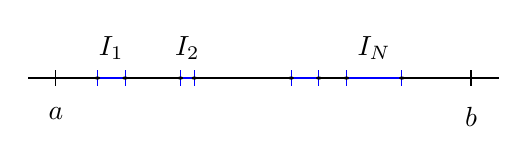
\begin{tikzpicture}[x=50]
       \draw (-1.2,0) -- (2.2,0);      
       \draw (-1, 0) node[below=7pt] {$a$};
       \draw[] (-1,-0.1) -- (-1,0.1);
       \draw (2, 0) node[below=7pt] {$b$};       
       \draw[] (2,-0.1) -- (2,0.1);
       
       \foreach \x in {-0.7,-0.5,-0.1,0, 0.7,0.9,1.1,1.5} {
        \draw[blue] (\x,-0.1) -- (\x,0.1);
    }
     \draw[blue, thick] (-0.7,0) -- (-0.5,0);
    \fill (-0.7,0) circle (0.02);
     \fill (-0.5,0) circle (0.02);
     
     \draw[blue, thick] (-0.1,0) -- (0,0);
    \fill (-0.1,0) circle (0.02);
     \fill (0,0) circle (0.02);
     
     \draw[blue, thick] (0.7,0) -- (0.9,0);
    \fill (0.7,0) circle (0.02);
     \fill (0.9,0) circle (0.02);
     
     \draw[blue, thick] (1.1,0) -- (1.5,0);
    \fill (1.1,0) circle (0.02);
     \fill (1.5,0) circle (0.02);
     
     \draw (-0.6, 0) node[above=3pt] {$I_1$};
     \draw (-0.05, 0) node[above=3pt] {$I_2$};
     \draw (1.3, 0) node[above=3pt] {$I_N$};
     
   \end{tikzpicture}$$

Con este recubrimiento finito, generamos una partición formada por $a$, $b$ y todos los extremos de los intervalos $I_j$ que denotaremos por $P$. Dicha partición, la expresaremos en términos de otras dos: $P_1$ que será la formada por los intervalos de la partición $P$ contenidos en algún $I_j$ y $P_2$ formada por los otros (que en particular no cortan a $D_{\varepsilon}$, luego la oscilación en estos es $<\varepsilon$). De este modo, tenemos $P = P_1 \cup P_2$.

Para cada intervalo $I\in P_2$, realizamos el siguiente procedimiento:
$$\forall I \in P_2:  \left(x \in I \Rightarrow o\left(f, x\right) < \varepsilon\right) \Rightarrow \exists I_x \subset I: \forall y, z \in I_x: \vert f\left(y\right) - f\left(z\right) \vert < \varepsilon$$
Y esto puede hacerse porque para cada $x$, podemos encontrar un $\delta$ de forma que en $(x-\delta, x+\delta)$ la oscilación es menor que $\varepsilon$ y precisamente ese sería un posible $I_x$.

Recubrimos $I$ (que es compacto por ser cerrado) por una cantidad finita de estos $I_x$ y, de esta manera, obtenemos en forma de partición (quitando trozos de intervalos si fuese necesario para que sean disjuntos) el intervalo $I$ inicial. Esto, genera otra partición de la parte que correspondía a $P_2$ que denotamos por $P^*_2$ y definimos $P^* := P_1 \cup P_2^*$ como nueva partición del intervalo.

De este modo, tenemos que:
$$U\left(f, P^* \right) - L\left(f, P^*\right) = \sum_{I\in P^*} \left(\sup_{x \in I} f \left(x\right) - \inf_{x \in I} f\left(x\right) \right) \mu\left(I\right) = $$
$$=\sum_{I \in P_1} \left( \sup_{x \in I} f \left(x\right) - \inf_{x \in I} f\left(x\right) \right) \mu\left(I\right) + \sum_{I \in P_2^*} \left(\sup_{x \in I} f \left(x\right) - \inf_{x \in I} f\left(x\right) \right) \mu\left(I\right) \le $$
$$ \leq 2M\varepsilon + \varepsilon\left(b - a\right) = \left(b - a + 2M\right) \varepsilon$$
Por el Criterio de Cauchy, $f$ es integrable Rienmann.

\item $\Rightarrow:$ supongamos que $f$ es integrable Riemann.

Como $D = \bigcup_{n \in \mathbb{N}} D_{\frac{1}{n}}$, basta con ver que $\forall n \in \mathbb{N}: \mu\left(D_{\frac{1}{n}}\right) = 0$. Para ello, tomamos $\varepsilon > 0$ y una partición $P$ de $\left[a, b\right]$ de forma que $U\left(f, P\right) - L\left(l, P\right) < \frac{\varepsilon}{n}$.

Denotamos por $P_1$ a los intervalos de $P$ que cortan a $D_{\frac{1}{n}}$ (con esto estamos asumiendo que los puntos de $D_{\frac{1}{n}}$ no son puntos de los extremos de la partición, pero no pasaría nada porque ese conjunto es de medida nula y la integral es la misma). De este modo, tenemos que:
$$\frac{\varepsilon}{n} > \sum_{I \in P_1} \left(\sup_{x \in I} f\left(x\right) - \inf_{x \in I} f\left(x\right) \right) \mu\left(I\right) \ge \frac{1}{n} \sum_{I \in P_1} \mu\left(I\right)$$
Sin embargo, esto quiere decir que:
$$\sum_{I \in P_1} \mu\left(I\right) < \varepsilon \mbox{ pero } D_{\frac{1}{n}} \subset \bigcup_{I \in P_1} I \Rightarrow \mu\left(D_{\frac{1}{m}}\right) = 0$$
\end{itemize}
\end{demo}

\begin{prop}
Si una función $f$ es integrable Riemann, entonces dicha función también es medible.
\end{prop}
\begin{demo}
Por el teorema de antes, $\mu(D) = 0$ lo que implica que $f$ es continua en c.t.p. y, por tanto, es medible.
\end{demo}
